\documentclass[12pt,a4paper,onecolumn,oneside]{extreport}

%/usr/texbin/latex -interaction=nonstopmode %.tex|/usr/texbin/bibtex %.aux|/usr/texbin/latex -interaction=nonstopmode %.tex|/usr/texbin/latex -interaction=nonstopmode %.tex

%\usepackage{times}
\usepackage{amsmath}
\usepackage{amssymb}
\usepackage[utf8x]{inputenc}
\usepackage[T1]{fontenc}
\usepackage[polish]{babel}
\usepackage{graphicx}
\usepackage{url}
\usepackage[ruled, vlined, polish]{algorithm2e-pl}
\usepackage{setspace}
\usepackage{tocbibind}
\usepackage{fancyhdr} 
\usepackage{eucal}  
\usepackage{rotating}
\usepackage{titlesec}
\usepackage{listings}
\usepackage{caption}
\captionsetup[lstlisting]{labelsep=none}
\usepackage{array}

\titleformat{\chapter}[display]{\normalfont\huge\bfseries}{\chaptertitlename\ \thechapter.}{20pt}{\vspace{-0.5cm}\huge} 


\setlength{\paperheight}{297mm}
\setlength{\paperwidth}{210mm} 

\setlength{\hoffset}{0.00cm}
\setlength{\voffset}{0.00cm}

\setlength{\oddsidemargin}{1.00cm}
\setlength{\topmargin}{1mm}
\setlength{\textheight}{\paperheight}
\textheight 22 cm	%26
\voffset -1.5 cm		%-3
\setlength{\textwidth}{16cm}  
\hoffset -0.5 cm
\setlength{\marginparsep}{1mm}  
\setlength{\marginparwidth}{2cm}
\setlength{\footskip}{2.36cm}   

\linespread{1.5}

% dzielenie wyrazów

\hyphenpenalty=2000			% nie dziel wyrazów zbyt często
\clubpenalty=10000			% kara za sierotki
\widowpenalty=10000			% nie pozostawiaj wdów
\brokenpenalty=10000		% nie dziel wyrazów między stronami
\exhyphenpenalty=999999		% nie dziel słów z~myślnikiem
\righthyphenmin=4			% dziel minimum 3 litery

\tolerance=4500
\pretolerance=250
\hfuzz=1.5pt
\hbadness=1450

\sloppy						% umacnia pozycję prawego marginesu


% Alter some LaTeX defaults for better treatment of figures:
% See p.105 of "TeX Unbound" for suggested values.
% See pp. 199-200 of Lamport's "LaTeX" book for details.
%   General parameters, for ALL pages:
\renewcommand{\topfraction}{0.9}	% max fraction of floats at top
\renewcommand{\bottomfraction}{0.8}	% max fraction of floats at bottom
%   Parameters for TEXT pages (not float pages):
\setcounter{topnumber}{2}
\setcounter{bottomnumber}{2}
\setcounter{totalnumber}{4}     % 2 may work better
\setcounter{dbltopnumber}{2}    % for 2-column pages
\renewcommand{\dbltopfraction}{0.9}	% fit big float above 2-col. text
\renewcommand{\textfraction}{0.07}	% allow minimal text w. figs
%   Parameters for FLOAT pages (not text pages):
\renewcommand{\floatpagefraction}{0.7}	% require fuller float pages
% N.B.: floatpagefraction MUST be less than topfraction !!
\renewcommand{\dblfloatpagefraction}{0.7}	% require fuller float pages

% arabskie 
% \renewcommand{\theequation}{A-\arabic{equation}}

\graphicspath{./img/}
\usepackage{wrapfig}
\begin{document}

% komenda \degree (kąt)
\newcommand{\degree}{\ensuremath{^\circ}}

% obrazki w~wyzszej rozdzielczosci
\def\imagesdraft{d}
\def\imagesoriginal{o}
\edef\imagesversion{\imagesoriginal}
%\edef\imagesversion{\imagesdraft}

\begin{titlepage}
	\begin{center}
	\vspace{3cm}
	\fontsize{25pt}{31pt}\selectfont
	POLITECHNIKA BIAŁOSTOCKA \\
	\vspace*{.5\baselineskip}
	\fontseries{b}\fontsize{24pt}{18pt}\selectfont
	Wydział Informatyki

	\vspace*{3\baselineskip}
	\fontseries{m}\fontsize{32pt}{20pt}\selectfont
	Paweł Żukowski\\
	\vspace*{\baselineskip}
	\fontseries{b}\fontsize{20pt}{15pt}\selectfont
	Projekt i~implementacja narzędzia do masowej refaktoryzacji identyfikatorów plików z~uwzględnieniem ich zawartości\\
%	Multifile Renaming Utility\\
%	Program narzędziowy do grupowej zmiany nazw plików na podstawie metadanych w~nich zawartch\\
	\vspace*{\baselineskip}
	\fontseries{m}\fontsize{15pt}{18pt}\selectfont
	PRACA INŻYNIERSKA \\
	\end{center}
	\vspace*{\baselineskip}
%	\begin{center}
%	wersja: template 16 X 2012
%	\end{center}
	\vspace*{3\baselineskip}
	\begin{flushright}
	\fontseries{m}\fontsize{18pt}{10pt}\selectfont
	Promotor\\
	dr inż. Marcin Skoczylas\\
	\end{flushright}
	
	\vspace*{4\baselineskip}
	\begin{center}
	Białystok 2013
	\end{center}

%
% sentencja na otwarcie pracy
%
%\newpage
%\thispagestyle{empty}
%\pagestyle{empty}
%\vspace*{20\baselineskip}
%
%\begin{flushright}
%
%\textit{Bardzo mały organizm nie może być piękny; jego obraz jest mylny, obiekt widoczny jest prawie niedostrzegalnie krótko. Zatem, czy ogromne może być piękne, skoro oko nie może zupełnie naraz ogarnąć całości, a~jednostkę oraz sens całości widz po prostu gubi?}
%
%\vspace{0.5cm}
%Arystoteles, Poetyka (około 335 p.n.e.)
%
%\end{flushright}

\end{titlepage}


\setcounter{page}{2}
%\chapter*{Podziękowanie}
%\huge \textbf{Podziękowanie}
%\vspace{2cm}

\textbf{Praca, której efektem jest niniejsza praca powstała przy wsparciu:}

\begin{itemize}
\item wsparcie 1
\item wsparcie 2
\item grant XXX
\end{itemize}

%\vspace{1cm}
\textbf{Autor zwraca się z uprzejmą prośbą, by jego serdeczne podziękowanie zechciały przyjąć wymienione niżej osoby:}

\begin{itemize}

\item prof. Abcdef Ghijkl 

\end{itemize}



\clearpage

\begin{center}
\textbf{Streszczenie}
\end{center}

\par
Niniejsza praca inżynierska na temat ''Projekt i implementacja narzędzia do masowej refaktoryzacji identyfikatorów plików z uwzględnieniem ich zawartości'' opisuje projekt architektury oraz implementacje programu Multifile Renaming Utility.
\par
Multifile Renaming Utility --- w skrócie MRU --- jest programem narzędziowym mającym na celu umożliwienie automatycznej zmiany nazw wielu plikom ze względu na metadane w nich zawarte.

\par
Praca jest podzielona na sześć rozdziałów zawierających teoretyczny jak i praktyczny opis problemu i jego rozwiązania.\\
Pierwszy rozdział zawiera wstępny opis projektu i motywacje do jego utworzenia.\\
Drugi rozdział zawiera teoretyczne podstawy problemu oraz opisuje terminologię użytą w pracy.\\
Trzeci rozdział przedstawia przykłady istniejących aplikacji wraz z ich subiektywną oceną pod względem skuteczności w stosunku do przedstawionego problemu.\\
Czwarty rozdział opisuje środowisko pracy, które zostało wykorzystane do stworzenia implementacji.\\
Piąty rozdział zawiera opis architektury, a także szczegóły implementacji gotowej aplikacji.\\
Ostatni, szósty rozdział składa się z wniosków na temat wykonanego projektu.

\vspace*{\baselineskip}

\noindent\textbf{Słowa kluczowe:} system plików, wtyczki, metadane, wxWidgets, boost, SigC++, C++

\clearpage

\begin{center}
\textbf{Summary}
\end{center}

\par
Following Engineer's Degree Thesis, titled ''Project and implementation of content aware, file renaming tool'' describes architecture project and implementation of Multifile Renaming Utility software program.

\par
Multifile Renaming Utility --- MRU for short --- is a tool application which aims to allow the user to rename many files based on metatdata contained therein.

\par
This thesis is divided into six chapters containing theoretical and practical description of the problem and its solutions.\\
First chapter contains introdution to the project and motivation which led to its creation.\\
Second chapter describes theoretical fundaments of described problem and terminology used in the work.\\
Third chapter is a review of few existing applications that aim to solve described problem.\\
Fourth section introduces work environment in which application were developed.\\
Fifth chapter contains architecture description as well as implementation details of the finished application.\\
The last, sixth chapter consists of the conclusions made ​​about the project.

\vspace*{\baselineskip}

\noindent\textbf{Keywords:} filesystem, plugins, metadata, wxWidgets, boost, SigC++, C++


\tableofcontents

\chapter{Wstęp}

\par
Z każdym rokiem ludzie oraz same komputery generują coraz większą ilość informacji.
Mimo że duża część z nich jest przechowywana w dobrze strukturyzowanych bazach danych, to ciągle, większość ludzi ma bezpośredni dostęp jedynie to tego co przechowuje w systemie plików własnego komputera.
<Rodzaje danych, ich zastosowanie>

\par
Od dziesięcioleci dysk twardy pozostaje głównym kontenerem dla danych użytkowników komputerów na całym świecie.
<Dane przechowywane w systemach plików>

\par
<Systemy plików, ich cechy wspólne, ograniczenia, metadane>

\par
<problem z identyfikatorami>

\clearpage

\section{Cel i zakres pracy}
\par
Niniejsza praca ma na celu stworzenie programu narzędziowego pozwalającego na automatyczne generowanie identyfikatorów (nazw) plików na podstawie metadanych w nich zawartych. <także danych generowanych przez sam program - CRC np>

\par
Zakres pracy obejmuje:
\begin{itemize}
\item Przegląd istniejących rozwiązań - programów i technik wspomagających masową zmianę identyfikatorów plików.
\item Porównanie funkcjonalności istniejących narzędzi i ich ograniczeń.
\item Projekt oraz implementacja wieloplatformowej architektury modułów.
\item Stworzenie parsera wyrażeń zawierających metatagi.
\item Projekt graficznego interfejsu użytkownika opartego na bibliotece wxWidgets.
\item Implementacja backendu do systemu plików opartego na bibliotece boost::filesystem.
\item Implementacja przykładowych modułów metatagów.
\item Testy aplikacji.
\end{itemize}

\section{Założenia}
Gotowa aplikacja powinna być niezależna od systemu operacyjnego w stopniu w jakim pozwalają na to zależności użytych bibliotek. Dzięki modułowej budowie powinna także udostępniać interfejs pozwalający na jej łatwą rozbudowę.

\section{Plan pracy}
<Co w jakim rozdziale się znajduje>
%W rozdziale \ref{teoria-identyfikatory} oraz~\ref{teoria-metadane} opisano Lorem ipsum dolor sit amet.

\clearpage

\chapter{Teoria}
\label{teoria}
\par
W~niniejszym rozdziale postaram się przybliżyć problem identyfikatorów plików opisując środowisko w~którym występuje.

\section{Dane w~systemie komputerowym}
\par
Jednym z~podstawowych elementów systemu komputerowego jest jego pamięć. Od początku istnienia komputerów istniała potrzeba składowania danych wymaganych przy praktycznie każdych operacjach wykonywanych przez jednostkę centralną komputera. Jako że pierwsze systemy komputerowe były wykorzystywane do obliczeń typowo matematycznych, algorytmy na nich uruchamiane nie wymagały wielkich kontenerów na dane. W~tych czasach wbudowane rejestry oraz ulotna pamięć RAM zaspokajały potrzemy rynku. Jednak wraz z~rozwojem sprzętu i~algorytmów na nim uruchamianych pojawiła się potrzeba przechowywania coraz to większej ilości danych jak, a~także (dzięki zastosowaniu architektury von Neumanna) samych programów. Pojawiła się idea nieulotnej oraz bardziej pojemnej pamięci --- dysku twardego.\\

\par
Pojemności pierwszych dysków twardych stanowiły promil dzisiejszych jednostek toteż nie wymagały stosowania systemów plików --- były po prostu nieulotnym rozszerzeniem pamięci operacyjnej RAM. Jednak wraz ze zwiększeniem ich pojemności oraz generalizacją oprogramowania, pojawiła się potrzeba standaryzowania i~kategoryzacji przechowywanych na dyskach danych, która spowodowała powstanie systemów plików.

\section{Systemy plików i~identyfikacja danych}
\par
System plików stanowi warstwę abstrakcji między programami, a~danymi zapisanymi na nośniku --- dysku twardym, karcie pamięci czy też płycie CD. System plików jest metodą zapisu danych, schematem dzięki któremu programy nie muszą operować na surowych blokach bajtów lecz mogą korzystać z~bardziej wysokopoziomowych deskryptorów plików, węzłów bądź ścieżek dostępu.\\
Zwykle systemem plików zarządza system operacyjny, który to udostępnia odpowiedni API\footnote{API --- Application Programming Interface}, a~także kontroluje dostęp do danych ze względu na uprawnienia użytkownika, programu lub samego zasobu będącego podmiotem zapytania programu.\\

\par
Istnieje wiele typów oraz implementacji systemów plików, które można podzielić na dwie kategorie:

\begin{itemize}
\item tradycyjne - znajdujące zastosowanie przy przechowywaniu dowolnych (ogólnych) danych w~postaci plików
\item specjalne - dostosowane do specyficznych rozwiązań (jak na przykład bazy danych)
\end{itemize}

Oddzielną kategorię mogą stanowić zdobywające coraz większą popularność wirtualne systemy plików --- różnią się one od tradycyjnych i~specjalistycznych tym że nie przechowują danych fizycznie na nośniku, a~są raczej aplikacjami udostępniającymi (generującymi) struktury danych na żądanie programu. Przykładem takich systemów mogą być: \texttt{procfs} --- udostępniający dostęp do procesów systemowych i~ich atrybutów w~systemach rodzin GNU/Linux oraz BSD, czy też \texttt{NFS} (Network File System) --- pozwalający na dostęp do systemów plików znajdujących się na innych komputerach w~sieci\cite{website:filesystems-howto}.

\subsection{Katalogi i~ścieżki do plików}
\par
Niniejsza praca skupia się na problemie opisywania danych w~tradycyjnych systemach plików za pomocą tak zwanych ścieżek, które identyfikują zasób w~drzewie katalogów\cite{wiki:path}.

\par
Tradycyjne systemy plików pozwalają na przechowywanie danych w~drzewiastej strukturze danych zwanej drzewem katalogów. W~większości implementacji każdy węzeł takiego drzewa może być katalogiem albo plikiem albo dowiązaniem do innego węzła. Dodatkowo węzły katalogów jako jedyne mogę posiadać węzły podległe --- podkatalogi\cite{website:filesystems-howto}.\\
Każdy węzeł (prócz węzła-korzenia) jest identyfikowany przez unikalny względem węzła-rodzica identyfikator zwany nazwą pliku.\\
Lista kolejnych nazw odseparowanych przez umowny symbol stanowi ścieżkę do pliku.
Ścieżki mogą być rozwijane względem aktualnej pozycji w~drzewie katalogów bądź od jego korzenia, odpowiednio nazywa się je ścieżkami względnymi oraz bezwzględnymi.
Warto zauważyć iż struktura drzewa katalogów nie wymusza sposobu rozkładu danych w~systemie plików --- tak długo jak identyfikatory pozostają unikalne, pliki przez nie opisywane mogą znajdować się w~tym samym katalogu\footnote{W praktyce ilość plików które mogą należeć do jednego węzła zależy od implementacji.}.

\subsection{Różnice w~identyfikacji plików wśród różnych systemów operacyjnych}
\par
Format ścieżki do pliku narzucany jest niezależnie od zastosowanego systemu plików przez system operacyjny.

\par
Systemy kompatybilne ze standardem \texttt{POSIX}, takie jak Apple MacOS, rodzina BSD, a~także rodzina GNU/Linux używają drzew katalogów z~pojedynczym, nienazwanym korzeniem oznaczanym symbolem prawego ukośnika (slash)~---~'\texttt{/}' \cite{website:posix-standard}.\\
Symbol prawego ukośnika jest również używany jako separator elementów (poziomów) ścieżki i~nie może stanowić elementu identyfikatora węzła w~wymienionych środowiskach.\\
Przykład ścieżki zgodnej ze standardem \texttt{POSIX}:
\begin{center}
\texttt{/home/idlecode/projects/mru/doc/main.tex}
\end{center}

\par
Systemy operacyjne z~rodziny Windows korporacji Microsoft\footnote{Istnieje  więcej systemów operacyjnych używających podobnego schematu} wykorzystują natomiast lewy ukośnik (backslash) --- '\texttt{\textbackslash}' --- jako separator komponentów ścieżki oraz uniemożliwiają stosowanie większej ilości symboli w~nazwach.\\
Drzewo katalogów systemu Windows może posiadać kilka korzeni (po jednym dla każdego dysku/partycji) oznaczanych pojedynczymi, zwykle dużymi literami alfabetu łacińskiego. Litera dysku wraz z~symbolem dwukropka poprzedza właściwą ścieżkę do pliku:\\
\begin{center}
\texttt{C:\textbackslash Users\textbackslash idlecode\textbackslash My Documents\textbackslash Projects\textbackslash MRU\textbackslash doc\textbackslash main.tex}
\end{center}

\par
Dodatkowo w~przypadku obu\footnote{System MacOS nie posiada tego ograniczenia} wyżej wymienionych schematów, nazwy elementów nie mogą zawierać znaku zerowego (NUL --- o~kodzie heksadecymalnym \texttt{0x00}), który może zostać zinterpretowany jako koniec łańcucha znaków\cite{website:fixing-unix-linux-filenames}.

\par
Większość implementacji pozwala zawrzeć pełen zakres symboli (znaków) w~ścieżce za pomocą kodowań z~rodziny \texttt{UTF} przy czym pojedynczy identyfikator może mieć maksymalną długość 255 bajtów\cite{wiki:path}.
Warto tu zauważyć iż systemy z~rodziny Windows zachowują wielkość liter w~identyfikatorach lecz przy interpretacji ścieżek --- rozwijaniu ich do odpowiadających węzłów --- nie gra ona znaczenia. Takie zachowanie nie występuje w~systemach kompatybilnych ze standardem \texttt{POSIX}. Istnieje również możliwość stosowania ukośników prawych do rozdzielania komponentów ścieżki tak jak to ma miejsce w~systemach \texttt{POSIX}-owych.

\par
Istnieje jeszcze kilka schematów zapisu ścieżek, które nie zostały przybliżone ze względu na zakres niniejszej pracy.

\clearpage

\section{Metadane}
%Co to są metadane
\par
Metadane z~definicji są danymi opisującymi inne dane. Metadane stosowane są w~przypadkach gdy nie istnieje fizyczna możliwość dołączenia lub dodatkowe informacje są zbyt luźno powiązane z~opisywanymi danymi.
Przykładem metadanych mogą być karty biblioteczne --- informują one o~statusie i~historii książki nie będąc jej integralną częścią.

%Metadane na poziomie systemu plikow
\par
W~systemach plików, metadane dostarczają informacji o~plikach zapisanych w~drzewie katalogów.
Przykładem komputerowych metadanych może być wspominana wcześniej nazwa czy ścieżka do pliku, która nie jest jego integralną częścią --- może zostać zmieniona bez naruszania struktury przechowywanego dokumentu.
Dodatkowo systemy plików często dostarczają ogólnych (wspólnych dla każdego pliku) atrybutów takich jak jego rozmiar, czas utworzenia lub ostatniej modyfikacji czy też prawa dostępu.
\par
Ciekawym przykładem metadanych są rozszerzenia nazw plików --- sufiksy rozpoczynające się od ostatniego znaku kropki w~nazwie. Rozszerzenia odgrywały ważną rolę w~systemach operacyjnych korporacji Microsoft gdzie stanowiły integralną część nazwy i~pozwalały systemowi skojarzyć typ pliku z~programem go obsługującym. W~systemach \texttt{POSIX}-owych informacja o~typie pliku jest zwykle przekazywana wraz z~kontekstem uruchomienia aplikacji operującej na pliku toteż rozszerzenia (jeśli już są fragmentem nazwy) stanowią bardziej informacje dla użytkownika.

%Metadane w~plikach i~obok nich
\par
Niektóre formaty plików (szczególnie kontenery multimediów) pozwalają na integracje metadanych z~samym plikiem. Jako że pliki (zwłaszcza binarne) mogą stosować dowolną strukturę zapisu, nie istnieje ogólny algorytm wyciągnięcia zawartych w~ten sposób informacji.
%Na szczęście popularne formaty plików posiadają wiele implementacji bibliotek umożliwiających dostęp do danych w~nich zawartych.

\par
Do metadanych można zaliczyć także dane generowane, takie jak sumy kontrolne, które są wartościami liczonymi na podstawie zawartości samego pliku. Sumy kontrolne używane mogą być w~celu testów integralności lub identyczności.

\chapter{Przegląd istniejących rozwiązań}
\par
Jako że problem zmiany identyfikatorów plików znany już jest od lat, na rynku istnieje wiele aplikacji próbujących się z nim uporać. Wiele z istniejących rozwiązań zostało zaprojektowanych dla plików konkretnego typulub są modułami większych aplikacji lecz istnieje kilka\footnote{Aplikacje zostały wybrane ze względu na ich popularność i podejście do rozwiązania problemu} implementacji gotowych do ogólnego zastosowania.
\par
Poniżej zostały przedstawione trzy wybrane implementacje wraz z subiektywną opinią o nich.

\section{Bulk Rename Utility}
\begin{figure}[h]
\begin{center}
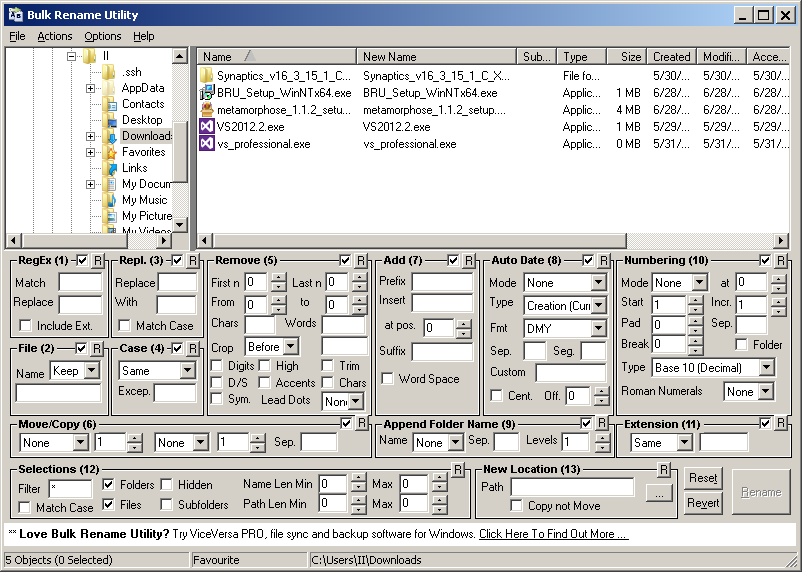
\includegraphics[scale=0.75]{img/bulkrename_window.png}
\end{center}
\caption{Okno główne programu Bulk Rename Utility}
\end{figure}

\par
Jednym z bardziej zaawansowanych i polecanych programów na platformę Microsoft Windows jest \textit{Bulk Rename Utility}. Aplikacja umożliwia ekstrakcje metadanych z plików audio (za pomocą tagów ID3v1) i obrazów zawierających dane EXIF, a także posiada wiele funkcjonalności związanych z modyfikacją istniejącej nazwy --- takich jak wyrażenia regularne.
Wyróżnia się wsparciem dla modyfikacji nazw i atrybutów katalogom, a także zwartym interfejsem .
Program nie wspiera zmiany kolejności wykonywania działań na nazwie --- wszystkie operacje mają swoją pozycje w kolejce wywołania i istnieje jedynie możliwość ich włączenia lub wyłączenia.
\textit{Bulk Rename Utility} posiada również swój odpowiednik --- \textit{Bulk Rename Command} --- który jest oddzielnym programem udostępniającym funkcjonalność programu z linii poleceń.

\section{Métamorphose}
\begin{figure}[h]
\begin{center}
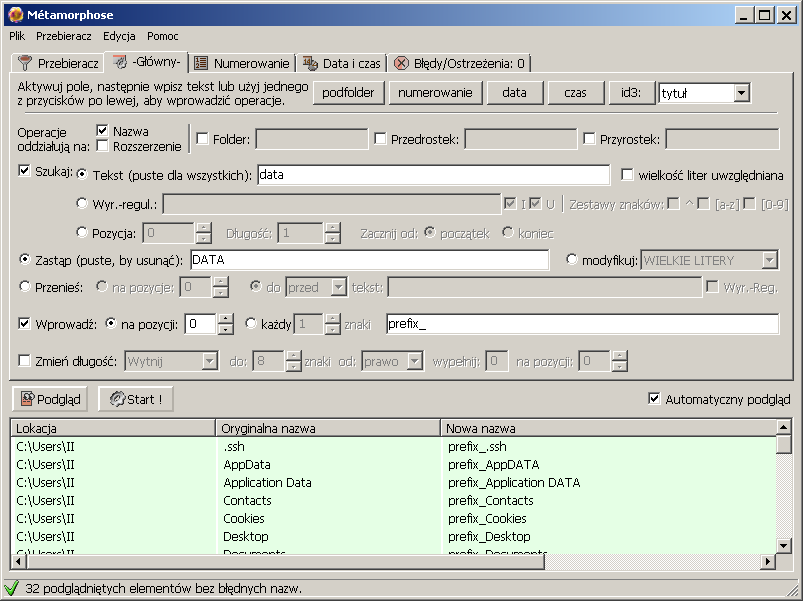
\includegraphics[scale=0.75]{img/metamorphose_window.png}
\end{center}
\caption{Jedna z zakładek programu Métamorphose}
\end{figure}

\par
\textit{Métamorphose} podobnie jak \textit{Bulk Rename Utility} korzysta z wbudowanego zestawu funkcjonalności jednak posiada pewne wsparcie dla szablonów nazw plików. Jest również aplikacją wieloplatformową, a także dzięki zastosowaniu zakładek --- bardziej przejrzystą.

\section{KRename}
\begin{figure}[h]
\begin{center}
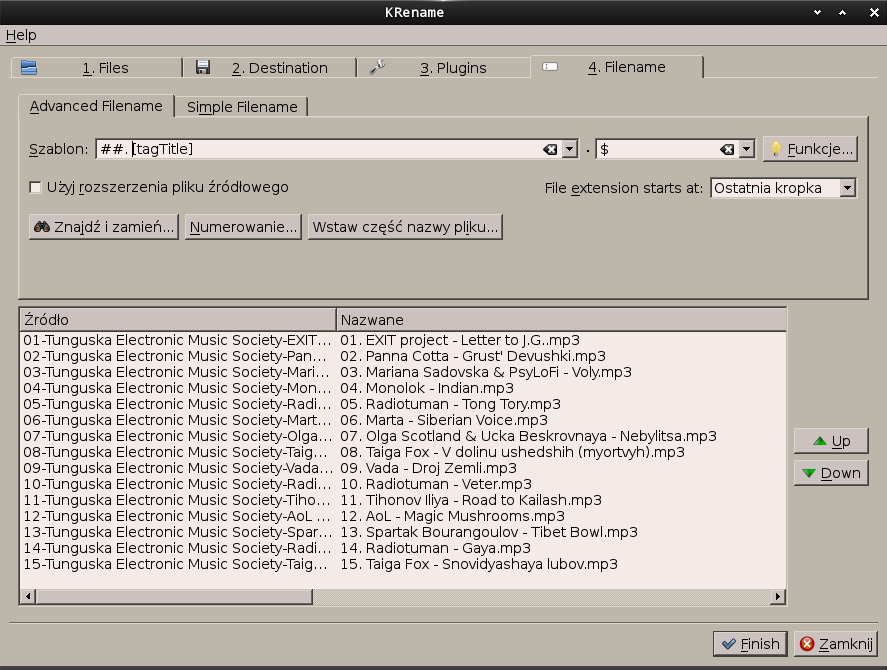
\includegraphics[scale=0.55]{img/krename_window.png}
\end{center}
\caption{Konfiguracja szablonu nazwy pliku w KRename}
\end{figure}

\par
\textit{KRename} w odróżnieniu od poprzednich programów nie posiada wersji dla systemów Windows. Zestaw zakładek pozwala na znalezienie plików, wybranie akcji do wykonania, a także przegląd i edycję wtyczek umożliwiających ekstrakcje danych. Poza trybem edycji szablonu dla nazw plików istnieje prostszy interfejs pozwalający na podstawowe operacje dodania sufiksu lub prefiksu, a także zmianę wielkości znaków w nazwie.\\
Zaletą programu jest duży wybór wtyczek pozwalających także na modyfikacje metadanych samych a nawet zawarcie w nowej nazwie rezultatu wywołania kodu JavaScript.

\section{Inne rozwiązania}
\par
Osoby korzystające z nowoczesnych systemów \texttt{POSIX}-owych posiadają ciekawą alternatywą dla jakichkolwiek specjalizowanych aplikacji --- tekstową powłokę zwaną shellem.\\
Nowoczesne powłoki shell takie jak \texttt{zsh} czy \texttt{bash} posiadają funkcjonalności umożliwiające łączenie wyników wywołań wielu komend co wraz z bogatą liczbą programów dostępnych dla wspomnianych systemów, umożliwia stworzenie polecenia które mogłoby w prosty modyfikować identyfikatory plików.

\begin{lstlisting}[label=shell-rename, caption={Polecenie powłoki zmieniające roszerzenia plików JPEG}]
find ./ -name *.JPG -exec rename -v 's/\.JPG/\.jpg/' {} \;
\end{lstlisting}

\par
Na listingu \ref{shell-rename} zostało pokazane przykładowe polecenie powłoki zamieniające rozszerzenia plików JPEG z '\textit{JPG}' na '\textit{jpg}'.
Wykorzystuje ono trzy programy:
\begin{itemize}
\item \texttt{find} --- znajduje pliki o rozszerzeniu kończącym się na '\textit{.JPG}' (przez zastosowanie parametru \texttt{-name *.JPG})
\end{itemize}
Polecenia realizujące proste zmiany nazw mogą zostać napisane przez średnio-wprawionego użytkownika powłoki jednak bardziej zaawansowane wymagają użycie wielu programów i nie są tak trywialne jak wyżej wymieniony przykład.

\chapter{Środowisko pracy}
%\label{srodowisko}
%\par
%Rozdział ten zawiera opis środowiska które zostało użyte do stworzenia i~testowania implementacji.

\section{Język C++}
\par
Aplikacja \texttt{MRU} została napisana przy użyciu języka C++ w~standardzie z~roku 2003 (ISO/IEC 14882:2003).
Język C++ jest dojrzałym, wieloplatformowym językiem programowania średniego poziomu, używanym od wielu lat przez programistów na całym świecie do tworzenia programów użytkowych, gier, sterowników czy nawet systemów operacyjnych. Dzięki kompatybilności z~C\footnote{C++ nie jest całkowicie kompatybilny z~C, jednak różnice w~obu tych językach są na tyle małe że rzadko wpływają negatywnie na kompatybilność (szczególnie na poziomie ABI).} pozwala na wykorzystanie wielu istniejących bibliotek napisanych zarówno w~C jak i~C++\cite{thinking-in-cpp}.

\subsection{LLVM Clang}
%\begin{wrapfigure}{r}{0.4\textwidth}
%\begin{center}
%
\includegraphics[scale=0.70]{img/clang_logo.png}
%\end{center}
%\caption{Logo frontendu Clang}
%\end{wrapfigure}
\par
\texttt{LLVM} --- Low Level Virtual Machine --- jest modułową architekturą do budowy kompilatorów. Pozwala ona na oddzielenie parserów różnych języków programowania od modułu optymalizacji (wspólnych dla wszystkich języków kompilowalnych) i~emiterów kodu bajtowego dla różnych platform.

\par
Clang jest parserem\footnote{Clang jest określany jako '\textit{frontend}' lecz słowo to nie ma dobrego odpowiednika w~języku polskim, a~główną funkcjonalnością tego narzędzia jest właśnie parsowanie plików źródłowych z~kodem C lub C++ do kodu pośredniego LLVM} języków C i~C++ dla architektury \texttt{LLVM}. Projekt jest otwarty (wydawany na licencji BSD) i~zdobywa coraz większą popularność\footnote{Od listopada 2012 Clang wraz z~LLVM stał się domyślnym kompilatorem dla systemu FreeBSD} dorównując, a~nawet przewyższając w~niektórych testach GCC\footnote{GNU Compiler Collection}.

\section{System operacyjny FreeBSD}
%\begin{wrapfigure}{l}{0.3\textwidth}
%\begin{center}
%
\includegraphics[scale=0.50]{img/freebsd_logo.png}
%\end{center}
%\caption{Logo systemu FreeBSD}
%\end{wrapfigure}
\par
System FreeBSD jest darmowym i~otwartym systemem operacyjnym z~rodziny BSD wywodzącej się z~rodziny \texttt{UNIX}-ów. Podobnie do dystrybucji GNU/Linux, sam w~sobie wraz z~wieloma, otwartymi bibliotekami tworzonymi przez społeczność stanowi środowisko przyjazne programistom.

\section{Mercurial}
\begin{wrapfigure}{r}{0.3\textwidth}
\begin{center}

\includegraphics[scale=0.50]{img/mercurial_logo.png}
\end{center}
\caption{Logo systemu Mercurial}
\end{wrapfigure}
\par
Do zarządzania plikami źródłowymi oraz kopią zapasową został wykorzystany rozproszony system kontroli wersji Mercurial wraz z~serwisem \url{bitbucket.org}. Narzędzie to pozwala na synchronizację kodów źródłowych między wieloma maszynami, ułatwiając tym samym pracę nad pojedynczym projektem wielu programistów.
\par
W~odróżnieniu od scentralizowanych systemów kontroli wersji takich jak SVN, Mercurial nie wymaga pojedynczego serwera, ani serwera w~ogóle. Pełne repozytorium może być trzymane na każdej maszynie z~której korzysta programista, a~praca różnych programistów może być synchronizowana bezpośrednio między nimi samymi\cite{version-control-example}.

\section{CMake}
\begin{wrapfigure}{r}{0.4\textwidth}
\begin{center}

\includegraphics[scale=0.75]{img/cmake_logo.png}
\end{center}
\caption{Logo narzędzia CMake}
\end{wrapfigure}

\par
Aby projekt był jak najbardziej przenośny i~niezależny od platformy, ważne jest aby jego proces budowania również taki był.
W~celu zapewnienia łatwego wsparcia dla budowania projektu na wielu platformach i~wielu łańcuchach narzędziowych, do budowania MRU został zastosowany CMake --- narzędzie do zarządzania procesem kompilacji i~zależnościami.
\par
CMake pozwala programiście określić z~jakich elementów składa się program i~jakich zewnętrznych zasobów (bibliotek) wymaga. Narzędzie następnie interpretuje skryptowy plik konfiguracyjny i~tworzy natywne dla danej platformy pliki projektowe zawierające odpowiednią do zbudowania projektu konfigurację.

\section{Vim}
\begin{wrapfigure}{r}{0.4\textwidth}
\begin{center}

\includegraphics[scale=0.25]{img/vim_logo.png}
\end{center}
\caption{Logo edytora Vim}
\end{wrapfigure}

\par
Edytor \texttt{Vim} jest rozszerzoną wersją klasycznego edytora \texttt{vi}, który jest standardowym oprogramowaniem w~przypadku dystrybucji zarówno GNU/Linux jak i~systemów z~rodziny BSD. Vim jest też platformą dla wielu pluginów które tworzą jego faktyczną funkcjonalność. Edytor sam w~sobie wspiera pracę z~wieloma dokumentami, koloruję składnie plików źródłowych i~posiada wiele komend ułatwiających produkcję kodu. Dzięki wtyczkom istnieje możliwość rozszerzenia go o~zaawansowane kompletowanie składni czy także szybkie wstawki kodu (ang. snippety).

\clearpage

\chapter{Implementacja}

\section{Specyfikacja wymagań}
\subsection{Wymagania funkcjonalne}
Użytkownikiem aplikacji jest administrator lub osoba posiadająca dużą kolekcję plików.
Wymagane funkcjonalności:
\begin{itemize}
\item Możliwość wyboru katalogu zawierających pliki wymagające zmiany nazw
\item Udostępnienie filtrów glob pozwalających na automatyczną selekcję plików
%\item Sortowanie wybranych plików za pomocą metawyrażeń
\item Możliwość ekstrakcji metadanych z plików typu
  \begin{itemize}
  \item MP3
  \item PNG
  %\item 
  \end{itemize}
\item Wybór operacji na samych plikach lub pełnych ścieżkach (wraz z katalogami)
\item Automatyczna iteracja względem wybranych plików i zmiana ich nazwy
\item Notyfikacja o powtarzających się identyfikatorach plików
\item Notyfikacja o możliwych problemach z kompatybilnością spowodowanych zastosowanym zestawem znaków
\item Notyfikacja o błędach ekstrakcji metadanych
\item Zachowywanie konfiguracji programu między uruchomieniami
\end{itemize}

\subsection{Wymagania niefunkcjonalne}
\begin{itemize}
\item Minimalistyczny, skalowalny interfejs użytkownika
\item Aplikacja powinna być przenośna na poziomie kodu źródłowego zarówno między platformami z rodziny Microsoft Windows jak i zgodnymi ze standardem \texttt{POSIX}.
\end{itemize}

\section{Projekt}


\section{Wykorzystane biblioteki}
\subsection{SigC++}
\begin{wrapfigure}{r}{0.4\textwidth}
\begin{center}

\includegraphics[scale=0.50]{img/sigcpp_logo.png}
\end{center}
\caption{Logo biblioteki SigC++}
\end{wrapfigure}
\par
SigC++ jest biblioteką dla języka C++ implementującą bezpieczny (ze względu na typy) mechanizm sygnałów.
Sygnały (zdarzenia) są wysokopoziomowym odpowiednikiem wywołań zwrotnych używanych do wstrzykiwania kodu programisty-użytkownika do istniejącej implementacji. W językach niskopoziomowych, takich jak C często stosuje się do tego celu wskaźniki do funkcji, jednak ich niskopoziomowa natura może powodować trudne do wykrycia błędy spowodowane przekazaniem złego typu wskaźnika lub błędnej jego sygnatury. Biblioteka udostępnia wysokopoziomowe szablony obiektów sygnałów jak i interfejsy do zastosowania w klasach użytkownika, ułatwiające w znaczny sposób zarządzanie podpiętymi zdarzeniami.\\
\par
SigC++ jest często używana w projektach GUI takich jak projekt pulpitu GNOME; w takim też celu zostanie ona użyta w aplikacji MRU.

\subsection{\texttt{boost::filesystem}}
\par
Biblioteka \texttt{boost::filesystem} pozwala na niezależny od systemu operacyjnego dostęp do drzewa katalogów. Ze względu na swoją uniwersalność została użyta jako podstawowy sterownik (moduł wyjścia --- output module) w aplikacji MRU.

\subsection{\texttt{boost::property\_tree}}
\par
\texttt{boost::property\_tree} jest drzewiastym (hierarchicznym) kontenerem ogólnego przeznaczenia\footnote{Z założenia biblioteka \texttt{boost::property\_tree} została stworzona do reprezentacji struktury ogólnych plików konfiguracyjnych lecz nic nie stoi na przeszkodzie aby traktować ją jako ogólny kontener}, który posłuży jako główne źródło informacji o wtyczkach i samym rdzeniu aplikacji MRU.

\subsection{\texttt{boost::program\_options}}
\par
Biblioteka \texttt{boost::program\_options} udostępnia wygodny i rozszerzalny parser argumentów przekazanych programowi z linii komend.

\subsection{wxWidgets}
wxWidgets jest wieloplatformową biblioteką do tworzenia graficznych interfejsów użytkownika (ang. GUI). W projekcie została wykorzystana do stworzenia wtyczki interfejsu (ui module) wxWidgetsUi. wxWidgets udostępnia i pozwala tworzyć przenośny zestaw klas kontrolek, które są tłumaczone na natywne kontrolki środowiska uruchamiającego aplikacje.

\subsection{ICU}
ICU --- International Components for Unicode" --- jest biblioteką opracowaną przez IBM wspierającą lokalizacje, globalizacje i umożliwiającą operacje na łańcuchach znaków w kodowaniach UTF.\\
Jako że główne operacje w aplikacji MRU przeprowadzane są na łańcuchach znaków, istotne jest aby wykonywane były one z należytą precyzją. ICU jest najbardziej zaawansowaną, ogólnie dostępną biblioteką tego typu z długą historią zastosowań.

\clearpage

\section{Rdzeń aplikacji - klasa MruCore}
Rdzeniem aplikacji jest klasa MruCore stanowi ona interfejs do całej funkcjonalności programu i udostępnia informacje o jego działaniu.
<!TODO!>

\section{Wyrażenia zawierające metatagi}
Najważniejszym elementem projektu MRU są metatagi wraz metawyrażeniami na które się składają.
Metawyrażenia używane są jak wzorzec (szablon) na podstawie którego generowane są kolejne nazwy plików.

\par
Za każdym razem gdy MRU zmienia plik na którym operuje, metawyrażenie jest ewaluowane. Każde wystąpienie tagu jest przekładane na wywołanie odpowiedniej metody na obiekcie wtyczki, a rezultat tego wywołania jest wstawiany w miejsce wystąpienia tagu.
Metatagi są reprezentacjami wywołań do odpowiadającym im wtyczek.

\begin{wrapfigure}{r}{0.4\textwidth}
\begin{center}

\includegraphics[scale=0.50]{img/metatag_sample.png}
\end{center}
\caption{Metatag z wyróżnionymi elemetami na niego się składającymi}
\end{wrapfigure}

\par
Metatag jest identyfikatorem wprowadzonym do zwykłego tekstu, składającym się z czterech elementów które nie mogą zostać rozdzielone białymi znakami. Metawyrażenie rozpoczyna się od symbolu procent --- '\%' --- po którym następuje nazwa metatagu składająca się ze znaków alfanumerycznych alfabetu łacińskiego\footnote{Z technicznego punktu widzenia nic nie stoi na przeszkodzie aby do zapisu nazwy metataga zastosować pełen zestaw znaków, lecz ze względu na globalizacje --- nie wszyscy użytkownicy potrafili by używać każdej nazwy --- zastosowano wyżej opisaną konwencję.}.
Po nazwie następuje para nawiasów --- '(' wraz z ')' --- zawierających opcjonalnie listę parametrów inicjalizacyjnych metatag. Nie istnieją ograniczenia co do zawartości listy inizjalizującej --- może ona zawierać pełen zakres znaków włączając to znaki zakończenia listy (nawiasy zamykające) o ile są odpowiednio oznaczone\footnote{Aby zignorować interpretację znaku specjalnego w metawyrażeniu, można użyć ogólnie znanego schematu wyłączania znaków --- poprzedzania ich symbolem '\textbackslash'}.
Ostatnim elementem jest opcjonalny zakres działania metatagu --- jest to obszar zawierający się między parą nawiasów klamrowych ('\{' oraz '\}') który sam w sobie jest metawyrażeniem. Dzięki temu, efekty metatagów mogą się na siebie nakładać.

\begin{figure}
\begin{center}

\includegraphics[scale=0.55]{img/metatag_expr.png}
\end{center}
\caption{Przykładowe metawyrażenie wraz z wyróżnionymi elementami metatagów}
\end{figure}

\par
Parsowanie metawyrażenia rozpoczyna się od tokenizacji --- wydzieleniu znaczących dla wyrażenia elementów takich jak symbole (procent, nawiasy), a także ciągi znaków alfanumerycznych oraz białych. Na podstawie listy tokenów budowane jest drzewo wywołań, które jest strukturą zawierającą kolejność oraz zależności między metatagami.
Drzewo wywołań składa się jedynie z metatagów. Aby otrzymać taką strukturę, ciągi surowego tekstu (nie będące metatagami) zostają zamienione na wywołania anonimowych (nienazwanych) metatagów, których argumentami inicjalizującymi są właśnie surowe ciągi tekstu, a jedyną funkcją --- zwrócenie argumentów z listy inicjalizującej. Dzięki temu ewaluacja wyrażeń jest prostsza, a dodatkowy anonimowy metatag może zostać wykorzystany na przykład do zmiany kodowania surowego tekstu.
\par
Wyrażenia są ewaluowane od lewej do prawej przy czym metawyrażenia zagnieżdżone w zakresach operacyjnych wyrażeń są ewaluowane przed otaczającym je metatagiem. W ten sposób rezultat wykonania pod-wyrażenia jest dostępny dla tagu-rodzica, co pozwala na wiązanie wywołań niespotykane w żadnym istniejącym programie.

\section{System modułów}
\par
Aby ułatwić proces projektowania a także zwiększyć rozszerzalność aplikacji, duża część funkcjonalności została oddelegowana do oddzielnych modułów zwanych również wtyczkami.
Wtyczki są klasami ładowanymi w trakcie działania programu z bibliotek dynamicznych.
W celu udostępnienia aplikacji funkcjonalności zawartych w modułach wtyczek, niezbędne było zaprojektowanie menadżera wtyczek --- plugin manager.
Klasy menadżera wtyczek umożliwiają programiście-użytkownikowi ładowanie modułów z wcześniej zadeklarowanym interfejsem niezależnie od platformy systemowej na której uruchamiany jest program\footnote{Same moduły muszą być skompilowane pod platformę na której program ma być uruchamiany.}.

\par
Problemem który rozwiązuje menadżer wtyczek jest fakt że biblioteki dynamiczne przechowują głównie funkcje; klasy które istnieją jedynie w trakcie kompilacji nie mogą zostać wyeksportowane do pliku jak ma to miejsce w językach wspierających introspekcje/refleksje typów --- takich jak Java czy C\#.
Aby umożliwić ładowanie wtyczek w języku C++ należy najpierw zdefiniować czym właściwie jest sama wtyczka.\\

W MRU (jak i wielu innych programach) wtyczka jest obiektem udostępniającym metody określone przez interfejs wtyczki. Także biblioteka dynamiczna musi w jakiś sposób udostępnić owe obiekty.

\par
Menadżer wtyczek po załadowaniu biblioteki dynamicznej przeszukuje ją pod kątem funkcji o nazwie \texttt{register\_plugins} wyeksportowanej bez przesłaniania nazw (name mangling) np za pomocą konstrukcji \texttt{extern "C" { ... }} i jeśli takowa istnieje --- uruchamia ją przekazując jako argument wskaźnik własną instancje.
\par
Sama wtyczka natomiast rejestruje w instancji przekazanego menadżera fabryki klas w niej zawartych.
Dzięki temu, obiekty wtyczek nie są tworzone od czas gdy są faktycznie potrzebne. Zmniejsza to obciążenie pamięciowe programu jak i ułatwia pracę twórcom wtyczek, którzy mogą skupić się na faktycznej implementowaniu faktycznej funkcjonalności modułów. Takie rozwiązanie pozwala również programowi-hostowi na decydowanie ile i kiedy mają być tworzone wybrane obiekty.

Z założenia menadżer wtyczek powinien umożliwiać ładowanie wielu wtyczek z jednej biblioteki dynamicznej.
Problem ten został rozwiązany dzięki zastosowaniu klasy identyfikatorów interfejsów --- każdy menażer i każda fabryka wtyczki posiada identyfikator informujący jaki typ interfejsu obsługuje. Dzięki zastosowaniu dystrybutora (brokera) fabryk, podczas ładowania modułu możliwe jest rejestrowanie fabryk wtyczek różnych interfejsów pod warunkiem że w czasie ładowania stworzone zostały ich instancje.

\section{Typy modułów w MRU} 
Aplikacja obsługuje trzy interfejsy wtyczek:
\begin{itemize}
\item UiPlugin - moduły interfejsu; pozwalają na implementacje różnych interfejsów użytkownika.
\item OutputPlugin - sterowniki wyjścia --- umożliwiają korzystanie z różnych interfejsów do systemu plików.
\item TagPlugin - moduły udostępniające fabryki do tworzenia wszelkich metatagów.
\end{itemize}

\section{Moduły UI}
\par
Wtyczki interfejsu użytkownika pozwalają użytkownikowi końcowemu na interakcję z programem.
Pojedynczy proces aplikacji może posiadać aktywną tylko jedną wtyczkę interfejsu. Decyzja o wyborze interfejsu użytkownika dokonywana jest na podstawie pliku konfiguracyjnego lub odpowiedniego przełącznika linii poleceń.
Wtyczki interfejsu odpowiadają za całkowitą komunikację między użytkownikiem i rdzeniem aplikacji --- MruCore; to one udostępniają większość funkcjonalności aplikacji, a także informują użytkownika o stanie programu.
\par
Jako że funkcjonalność aplikacji jest w dużej mierze determinowana przez klasę rdzenia (MruCore), interfejs UiPlugin nie posiada z góry zdefiniowanych metod jak inne wtyczki. Jedyna metoda w nim zawarta --- \texttt{start} --- pozwala na reinterpretacje linii poleceń i służy do przekazania kontroli nad programem (klasą MruCore) właśnie do samej wtyczki.

\subsection{wxWidgetsUi}
\par
wxWidgetsUi jest implementacją graficznego interfejsu użytkownika opartego na wspomnianej bibliotece \texttt{wxWidgets}. Założeniem tego modułu jest udostępnienie użytkownikowi końcowemu prostego oraz szybkiego dostępu do funkcjonalności programu, a także pomoc w zapoznaniu się z aplikacją.

\begin{figure}
\begin{center}
%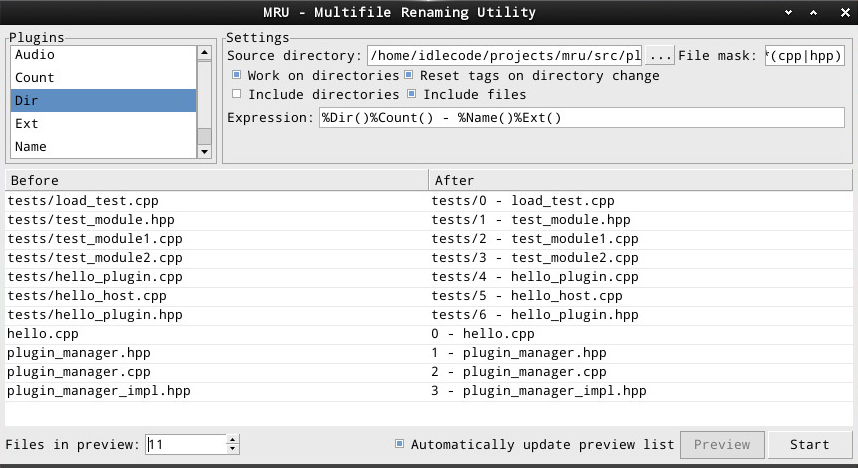
\includegraphics[scale=0.50]{img/wxwidgetsui.png}
\end{center}
\caption{Okno aplikacji MRU --- wtyczka wxWidgetsUi}
\end{figure}

Okno aplikacji stworzone przez wtyczkę wxWidgetsUi jest podzielone na trzy sekcje:
\begin{itemize}
\item Sekcja górna odpowiada za selekcję plików oraz pozwala na edycję metawyrażenia które ma zostać zastosowane na wybranych plikach.
W lewym górnym rogu widnieje lista dostępnych Metatagów, a pola po prawej stronie pozwalają na wybór katalogu, filtru glob oraz samego metawyrażenia.

\item Środkowa część okna stanowi podgląd wybranych plików jak i efektów zastosowania edytowanego wyrażenia do nich. Lista plików może być ograniczona i odświeżana w zależności od opcji znajdujących się pod nią.

\item Na dole okna widoczne są przyciski do (ręcznego) generowania podglądu, jego konfiguracji, a także rozpoczęcia transformacji nazw dla wybranych plików.
\end{itemize}

\subsection{TextUi}
\par
TextUi jest wtyczką interfejsu udostępniającą funkcjonalność programu z poziomu linii komend. Pozwala ona na przekazanie parametrów konfiguracyjnych i rozpoczęcie transformacji nazw bez interakcji z użytkownikiem jak ma to miejsce w przypadku graficznych interfejsów użytkownika. Dzięki zastosowaniu tej wtyczki istnieje możliwość wykorzystania aplikacji MRU z poziomu skryptów powłoki, na maszynach nie wykorzystujących środowiska graficznego lub zdalnych.

\section{Moduły output}
\par
Wtyczki wyjścia są warstwą abstrakcji pomiędzy systemem operacyjnym i jego drzewem katalogów, a rdzeniem aplikacji. Udostępniają one iteratory pozwalające na przeszukiwanie  dysku w celu znalezienia plików pasujących do wzorca wybranego przez użytkownika, oraz przekazują polecenia zmiany identyfikatora pliku do API używanego systemu. Kontrolują one również poprawność wygenerowanych nazw, a także zapewniają ich unikalność.

\subsection{GenericBoost}
Wtyczka GenericBoost została opracowana na podstawie biblioteki \texttt{boost::filesystem}. Stanowi ona sprawdzone oraz przenośne rozwiązaniem problemu dostępu do drzewa katalogów, bezpieczne do wykorzystania na wielu systemach bez zmian w kodzie samej wtyczki.


\section{Moduły metatagów}
Główna funkcjonalność aplikacji została zawarta w modułach tagów --- to one odpowiadają ekstrakcje metadanych lub generowanie wartości, które rdzeń aplikacji jedynie składa i przesyła wraz z komunikatem zmiany do systemu plików.
\par
Każdy z poniżej wymienionych tagów może zostać dodany do wyrażenia po załadowaniu odpowiedniej biblioteki dynamicznej go zawierającej\footnote{Część tagów nie wymaga ładowania --- są wbudowane w plik wykonywalny aplikacji, natomiast część mimo iż jest dostarczana w standardzie z aplikacją może wymagać dodatkowej konfiguracji w postaci określenia ścieżki ładowania bibliotek}.

\subsection{Count}
Tag Count jest używany do numeracji wybranych plików.
Dla każdego pliku generowany jest kolejny numer. Lista argumentów tagu pozwala na określenie wartości początkowej, prefiksu oraz systemu w którym ma odbywać się numeracja.
W poniższej tabeli zawarte zostały parametry obsługiwane przez metatag:
\begin{table}[h]
\begin{center}
\begin{tabular}{| c | p{13cm} |}
\hline
\textbf{Argument} & \textbf{Opis} \\
\hline
start=\textit{N} & Ustawia początkowy stan licznika na \textit{N}--- od tej wartości tag rozpocznie zliczanie \\
step=\textit{N} & Ustawia rozmiar kroku --- kolejny numer będzie większy o \textit{N} w stosunku do poprzedniego \\
\hline
\end{tabular} \end{center}
\caption{Zestaw argumentów inicjalizacyjnych dla metatagu Count}
\end{table}

Aby wykorzystać kilka argumentów jednocześnie należy oddzielić je od siebie za pomocą symbolu przecinka --- '\texttt{,}'.

\subsection{MP3}
Tag MP3 pozwala na ekstrakcję danych z plików audio zakodowanych w standardzie MPEG-1/MPEG-2 Audio Layer 3 oraz zawierających tagi ID3.
Tag ten obsługuje następujące argumenty:
\begin{table}[h]
\begin{center}
\begin{tabular}{| c | p{13cm} |}
\hline
\textbf{Argument} & \textbf{Opis} \\
\hline
title & Konfiguruje tag do ekstrakcji tytułu utworu \\
artist & Konfiguruje tag do ekstrakcji nazwy artysty wykonującego utwór \\
album & Konfiguruje tag do ekstrakcji nazwy albumu w którym zawiera się utwór \\
year & Konfiguruje tag do ekstrakcji roku powstania utworu \\
comment & Konfiguruje tag do ekstrakcji komentarza \\
\hline

\end{tabular}
\caption{Zestaw argumentów inicjalizacyjnych dla metatagu MP3}
\end{center}
\end{table}

\subsection{CRC32}
Metatg CRC32 służy liczenia cyklicznej sumy kontrolnej CRC o wielkości słowa 32 bity.
Zwracana suma kontrolna jest sformatowana jako wartość heksadecymalna.

\subsection{TextCase}
Tag TextCase jest używany do zmiany wielkości liter w skojarzonym z tagiem zakresie działania. Pewność działania dla pełnego zakresu kodów unicode jest zapewniona dzięki wykorzystaniu funkcji z biblioteki ICU.

\begin{table}[h]
\begin{center}
\begin{tabular}{| c | p{13cm} |}
\hline
\textbf{Argument} & \textbf{Opis} \\
\hline
upper & Konfiguruje tag do zamiany wszystkich znaków w zakresie na ich większe odpowiedniki \\
lower & Konfiguruje tag do zamiany wszystkich znaków w zakresie na ich mniejsze odpowiedniki \\
title & Konfiguruje tag do zamiany znaków w zakresie tak by wyglądały na tytuł (Pierwsze znaki każdego słowa są zamieniane na ich większe odpowiedniki \\
\hline
\end{tabular} \end{center}
\caption{Zestaw argumentów inicjalizacyjnych dla metatagu TextCase}
\end{table}

\section{Testy}

\chapter{Wnioski}
\label{wnioski}

\par
Wiele bibliotek i~szczegółów implementacji sprawiło że projekt pracy inżynierskiej okazał się nieco trudniejszy niż było to przewidywane.
Dużą częścią pracy stanowiło połączenie istniejących bibliotek i~technologii aby mogły ze sobą współpracować. Różnica zaawansowania oraz stylów interfejsów użytych narzędzi wymusiła tworzenie dodatkowych abstrakcji lecz dzięki temu, pozwoliła także na zmniejszenie zależności między-modułowych co zaowocowało powstaniem aplikacji o~dużych możliwościach rozwoju.
%Omówiona aplikacja może być dalej rozwijana jako projekt open-source.

\par
Również projekt architektury aplikacji okazał się nie tak prosty jak mogłoby to wynikać z~założeń. Aby móc stosować operacje działające na wielkich zbiorach danych, przepisany musiał zostać cały system wtyczek wejścia, który w~pierwszej po prostu wczytywał listę plików, a~w ostatecznej był kaskadą iteratorów.

\par
Nad wyraz ciekawym doświadczeniem okazał się również parser metawyrażeń.
 W~pierwszej wersji został on zaimplementowany w~sposób spójny i~monolityczny, jednak gdy zaszła potrzeba jego rozszerzenia, musiał zostać podzielony na bardziej niezależne moduły (tokenizera, leksera i~samego parsera). Zaowocowało to ciekawą architekturą, którą autor planuje rozwijać w~przyszłości.

\par
Stworzona aplikacja sprostała założeniom pod które została zaprojektowana i~stanowi dzięki temu użyteczne narzędzie które może pozwolić ludziom na to na co zostały stworzone komputery --- zautomatyzowanie monotonnych czynności i~przyspieszenie pracy.

\par
Dodatkową zaletą wykonanej aplikacji jest fakt że niektóre jej części (takie jak menadżer wtyczek) dzięki swojej uniwersalności mogą posłużyć do budowy kolejnych programów.


%%\chapter*{Definicje}
\chapter{Definicje}
\begin{list}{}{\leftmargin=0em}

\item $\mathbb{R}$ - zbiór liczb rzeczywistych
\item $I$ - macierz opisująca obraz wejściowy
\item $w$ - szerokość obrazu wejściowego, liczba kolumn macierzy $I$


\end{list}
%\chapter*{Lista publikacji}
\thispagestyle{empty}
\pagestyle{empty}

\par
\hspace{0.6cm}C. Zet, H. Kiesewetter, M. Skoczylas, L. Westerberg, R. Spohr. A system for irradiating polymer films with a preset number of ions. GSI Scientific Report, Gesellschaft f\"ur Schwerionenforschung mbH (GSI), 154, 2003

\par
C. Zet, C. Foslau, M. Skoczylas, L. Westerberg, R. Spohr. System for irradiating polymer films with a preset number of ions. SIELMEN, 4th International Conference on Electromechanical and Power Systems  vol. 2, 167-170, 2003

\par M. Skoczylas, K. Andrzejewski. Krzyżtopór. Telewizja Polska, wyd. Rzeczpospolita, Akademia Filmu i Telewizji Warszawa, 2005



\bibliography{references}
\nocite{*}
%\bibliographystyle{plain}
\bibliographystyle{unsrt}

\end{document}

